
%%%%%%%%%%%%%%%%%%%%%%% file typeinst.tex %%%%%%%%%%%%%%%%%%%%%%%%%
%
% This is the LaTeX source for the instructions to authors using
% the LaTeX document class 'llncs.cls' for contributions to
% the Lecture Notes in Computer Sciences series.
% http://www.springer.com/lncs       Springer Heidelberg 2006/05/04
%
% It may be used as a template for your own input - copy it
% to a new file with a new name and use it as the basis
% for your article.
%
% NB: the document class 'llncs' has its own and detailed documentation, see
% ftp://ftp.springer.de/data/pubftp/pub/tex/latex/llncs/latex2e/llncsdoc.pdf
%
%%%%%%%%%%%%%%%%%%%%%%%%%%%%%%%%%%%%%%%%%%%%%%%%%%%%%%%%%%%%%%%%%%%


\documentclass[runningheads,a4paper]{llncs}

\usepackage{amssymb}
\setcounter{tocdepth}{3}
\usepackage{graphicx}
\usepackage{rotating}

\usepackage{url}
\urldef{\mailsa}\path|kruza@ufal.mff.cuni.cz|    
\newcommand{\keywords}[1]{\par\addvspace\baselineskip
\noindent\keywordname\enspace\ignorespaces#1}

\begin{document}

\mainmatter  % start of an individual contribution

% first the title is needed
\title{Mitigating Low Audio Quality by Domain Transfer for Better ASR}

% a short form should be given in case it is too long for the running head
\titlerunning{Audio Domain Transfer for Better ASR}

% the name(s) of the author(s) follow(s) next
%
% NB: Chinese authors should write their first names(s) in front of
% their surnames. This ensures that the names appear correctly in
% the running heads and the author index.
%
\author{Jan Oldřich Krůza}
%
\authorrunning{Jan Oldřich Krůza}
% (feature abused for this document to repeat the title also on left hand pages)

% the affiliations are given next; don't give your e-mail address
% unless you accept that it will be published
\institute{Institute of Formal and Applied Linguistics,\\
Faculty of Mathematics and Physics,\\
Charles University
\mailsa\\
\url{ufal.mff.cuni.cz}}

%
% NB: a more complex sample for affiliations and the mapping to the
% corresponding authors can be found in the file "llncs.dem"
% (search for the string "\mainmatter" where a contribution starts).
% "llncs.dem" accompanies the document class "llncs.cls".
%

\toctitle{Mitigating Low Audio Quality by Domain Transfer for Better ASR}
\tocauthor{Jan Oldřich Krůza}
\maketitle


\begin{abstract}
The paper presents an attempt to solve the problem of bad audio quality
affecting the accuracy of speech-to-text systems. I
describe an experiment with Gycle-GAN domain transfer from the defect to the
pure as a way to reduce the impact of noise, overdrive, reverberation and other
defects.
\keywords{speech recognition, GycleGAN, domain transfer, signal processing}
\end{abstract}

\section{Introduction}

Automatic speech recognition is generally approached by means of machine
learning: a statistical model is inferred based on some training data. Its
application bases on the assumption that whatever was learned about the training
data will also apply for the input data. It is clear then, that if the input
data have different properties than the training data, the basic assumption is
violated and the inference performance will suffer.
Also if the training data themselves are damaged in a way that makes the desired
information harder to extract, the learning is going to be less successful.

For speech recognition, the problem of noise, reverberation and other defects
has been a pain point and also a point of research. To mention some, Gillespie
and Atlas\cite{gillespie2002diversity} deal with reverberation for
GMM-based ASR, Yoshioka et al.\cite{reverbmagazine} summarize various
dereverberation techniques, Ko et al.\cite{reverbaugment} attempt to
simlulate reverberation in training data digitally. Seltzer, Yu and
Wang\cite{dnnnoiserobust} deal with noise in DNN-based ASR.

There are in principle two ways to deal with the negative effect of acoustic
deficiencies in speech recognition: 1) to adapt the model, which includes
training on augmented data, and 2) to adapt the input data. This article
presents an experiment in the latter approach.

\section{Spoken Corpus of Karel Makoň}

I am looking into the problem of acoustic inconsistencies in terms of varying
overall quality, reverberation, noise, overdrive and other phenomena in a
dataset that is to be automatically transcribed and listened to by humans.

The application is at the spoken corpus of Karel Makoň\cite{makondata}, for which
a speech recognition system has been developed\cite{kruuza2012making} but where
the heterogenous acoustic quality affects both the speech recognition
performance and the listening experience. Whereas the word error rate on the
overall test set is 21\%, it is 45\% on a sample of recordings suffering from
overdrive, and 68\% on recordings taken on a magnetophone tape with a slow
recording speed of 2 centimeters per second after some 30 years of living-room
storage.

I am conducting an experiment to make the input data similar to the training
data instead of the more usual other way around because 1) it is not easy to
make the volunteer annotators transcribe acoustically flawed data, 2) a
success would not only benefit speech recognition results but also listening
experience and 3) the model could stay leaner.

What acoustic defects are actually present? Since the corpus was digitized from
magnetophone tapes of spontaneous talks by a single speaker recorded in various
amateur conditions and with consumer devices, we can broadly distinguist these
types of interefering signal:
\begin{enumerate}
\item{additive noise -- hum or hiss,}
\item{
    stationary interference like screeching added by low-quality magnetophone
    parts or the erasing head signal,
}
\item{non-stationary interference like background speech or door slams,}
\item{
    room echo or ill-equalized microphone boosting or cutting certain
    frequencies,
}
\item{non-linear distortion of the magnetophone}
\item{speed fluctuations.}
\end{enumerate}

The individual interference types affect each other and can occur several times
in several stages. For instance, echo is like a convolution with a certain
sample vector. It is followed by non-linear distortion and after that
convolution again with a different vector in the imperfect magnetophone
circuits. Additive noise comes on top of that. Another batch of distortions
comes during the playback. Clearly, modeling, let alone reverting these
interferences is a difficult task.

\section{Neural Domain Transfer}

The revolutionary article of Zhu et al.\cite{cyclegan} presenting
cycle-consistent generative adversarial networks gave mankind a mighty tool and
a hilarious toy that was used for de-hazing
photographs\cite{Engin_2018_CVPR_Workshops}, giving people other's facial
expressions\cite{jin2017faceoff}, in biomedicine\cite{yang2018biogan} and also
in speech processing: Kaneko and Tameoka\cite{kaneko2017parallel} present
speech domain transfer and Hosseini-Asl et al.\cite{hosseini2018malevoicegan} do
the same for the purpose of speech recognition.


Most closely related to the work presented in this article is probably
SEGAN\cite{pascual2017segan}: CycleGAN employed to enhance speech.

CycleGAN assumes two datasets in consistent domains: day and night photos,
schematic and photographic maps, male and female speech etc. In this case,
we have a clear consistent domain of clean, high-quality recordings and the
rest, which suffers from any combination of a number of defects. The damaged
recordings are very unlike each other, they don't form a consistent domain.

There are two ways of dealing with this situation: 1) adapt CycleGAN so that it
can deal with a ``compact'' and a ``scattered'' domain or 2) cluster the
data and apply CycleGAN on the individual clusters. While adapting CycleGAN may be a
point of future work, I have explored the simpler way of clustering the data.

\section{Clustering}

In order to perform clustering on any dataset, a metric on the data is needed.
I have used that proposed by Mandel \& Ellis\cite{mandel2005song}, which
is based on mel-frequency cepstra. A distance matrix has been created using the
tool musly\cite{schnitzer2011using} and the clusters on top of that using
hierarchical clustering\cite{johnson1967hierarchical}.

A manual... or rather aureal check on the clusters confirms that files falling
into a cluster are indeed acoustically similar. So we arrived at a cluster of
overdriven recordings, a cluster of heavily hummed ones etc.

For curiosity, I looked at the distances of the files among each other and
compared it to that between other familiar sounds. For instance, two adjacent
segments of the same speaker from a meeting of the Czech parliament has a
distance of 1.4. Different speakers have a distance of 6.5. One of these
segments compared to a black metal song chorus has the distance of 519. On the
other hand, the median distance among the Spoken corpus of Karel Makoň, where
there is one single speaker, amounts to 55.9.

The experiment presented below is conducted on three clusters: 1) A cluster
of the cleanest recordings, used as the destination domain, 2) a cluster of
overdriven recordings and 3) one of those recorded with low tape speed. The
latter recordings are the hardest to understand also for humans. All clusters
have a maximum internal distance of 25.

\section{Results}

I have used the voice transfer method as proposed by Kaneko \&
Kameoka\cite{kaneko2017parallel} and implemented by
Mao\footnote{github.com/leimao/Voice\_Converter\_CycleGAN}. I have trained
transfer 1) between the clean and the overdriven cluster and 2) between the
clean and the low-speed cluster.

After 200 epochs, I have performed speech recognition on the transferred data.
The result is summed up in Table~\ref{tab:results}.

\begin{table}[htpb]
\begin{center}
\begin{tabular}{|l||r|r|}
\hline
           & original & transferred \\
\hline
overdriven & 0.450 & 0.441 \\
low-speed  & 0.685 & 0.939 \\
\hline
\end{tabular}
\caption{Word error rate for the two damaged clusters before and after CycleGAN
transfer.}\label{tab:results}
\end{center}
\end{table}

The small but apparent reduction in word error rate in case of the overdriven
cluster is the positive, promising result. The improvement is rather small, and
as such it does not seem worthwhile applying it on the entire corpus. It
proves, however, that there is some potential. An important immediate benefit is
that the transferred overdriven (or should I say de-overdriven) sound files are
much easier on the ear and it can be a help for the human listener.

The wrecking word error rate increase from 69\% to 94\% in case of the
recordings taken at low tape speed requires further investigation.
Figure~\ref{fig:plzen} shows the waveform and spectrum of a sample from the low-speed
cluster before and after the transfer. For comparison,
Figure~\ref{fig:overdrive} shows the same for the overdriven cluster.
Notice how parts of the signal are completely missing in the converted low-speed
sample. It seems that when the signal is too hard to separate from the noise,
the covertor prefers to generate silence.

\begin{figure}[htpb]
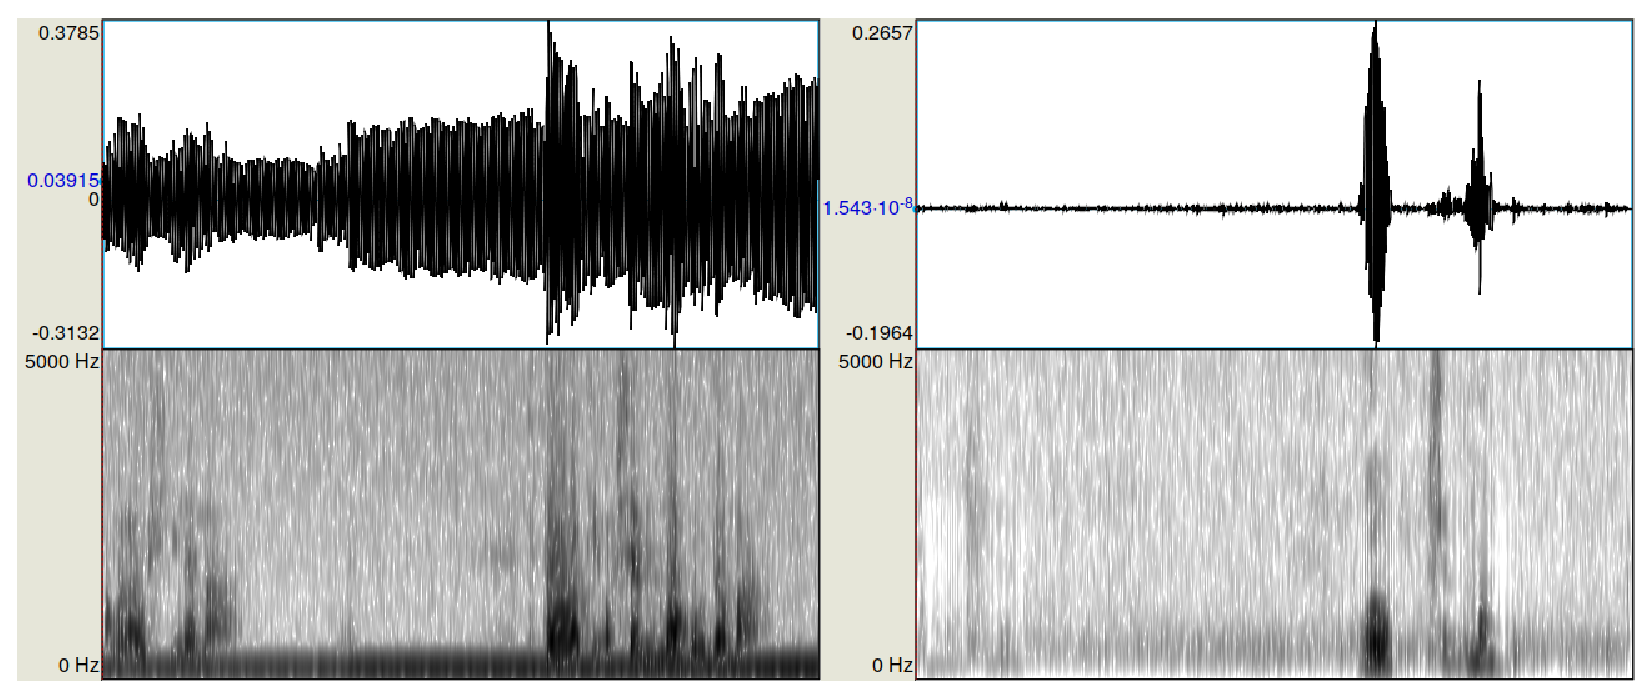
\includegraphics[scale=0.4]{rc/plzen.eps}
\caption{Wave form (above) and spectrogram (below) of a recording taken in low
tape speed before the CycleGAN transfer (left) and afterwards (right).}
\label{fig:plzen}
\end{figure}

\begin{figure}[htpb]
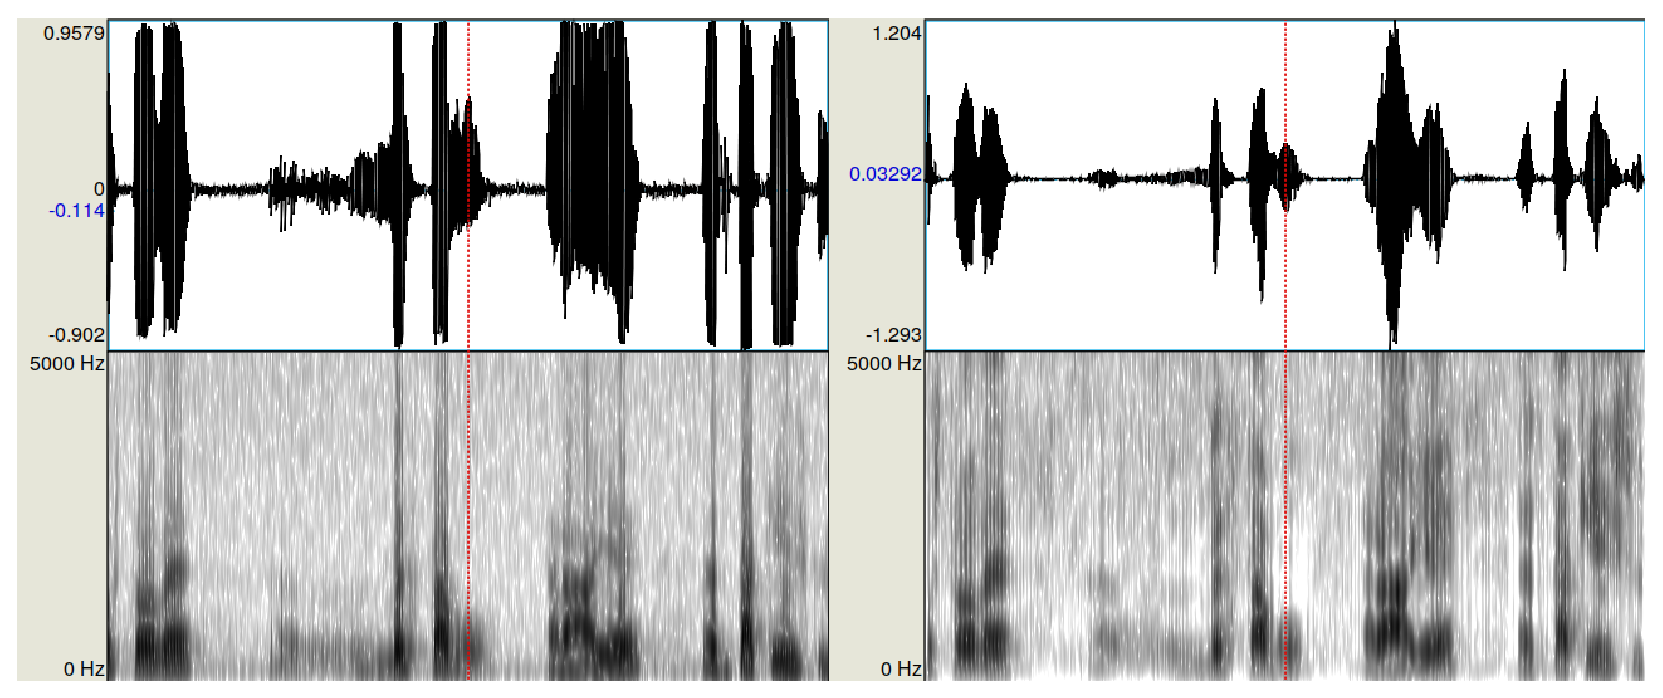
\includegraphics[scale=0.4]{rc/overdrive.eps}
\caption{Wave form (above) and spectrogram (below) of an overdriven recording
before the CycleGAN transfer (left) and afterwards (right).}
\label{fig:overdrive}
\end{figure}

%\subsection{Adapting CycleGAN for scattered domain}
%
%The way CycleGAN works given two datasets, one representing a domain $A$, the
%other representing a domain $B$, it learns two functions $f(A) -> B$ and
%$g(B) -> A$ that map the data between the two domains. In my case, where domain
%$B$ is not really a domain but more like a linear combination of several
%domains, the function $f$ that maps clean data to damaged data is not well
%defined. Indeed, how can we define a function that maps a clean recording to a
%damaged one when ``damaged'' can mean anything from overdrive, reverberation,
%noise, a frequency filter, and a number of other phenomena, and their
%combinations?
%
%A way could be to leverage the knowledge of the partially above listed possible
%effects that can turn a clean recording to a damaged one. If we defined
%elementary transformations simulating the individual ways a recording can be
%damaged, we could be looking for a linear combination of these transformations
%such that applying them on the clean sample $a \in A$ yields a result as similar
%to the damaged sample $b \in B$ as possible.
%
%Like this, we could make instead of $f(a \in A) -> B$ a function
%$f(a \in A, b \in B) -> B$ without the danger that it would degenerate to just
%returning the sample $b$.
%
%Aside of a metric for similarity between two sound files, we would need the list
%of transformations that take a substantial part in the acoustic damaging at
%hand.
%

\section{Conclusion}

Neural-network domain transfer offers a universally applicable method to
mitigate any kind of and combination of acoustic defects without the necessity
of modeling the specific effects.
The method was demonstrated to help to a small extent with speech recognition
results. However, where the damage is too severe, it discards the only
information at hand instead of improving its quality.

The benefit for human listeners seems quite promising although a quantitative
evaluation would be needed to assess it properly.

\section*{Acknowledgments}

This work has been using language resources developed, stored and distributed by
the LINDAT/CLARIAH project of the Ministry of Education, Youth and Sports of the
Czech Republic (project LM2018101).

\bibliographystyle{splncs}

\bibliography{citace}

\end{document}
